\chapter{Threat Model}

Security as part of a software project is nowadays an element that should no longer be neglected. When security is considered from the beginning of a project, it is much easier to keep pace of the evolving threat landscape, quickly derive implications in case of an emerging vulnerability and adapt the project where necessary. Another benefit is the significantly shorter time to react as identifying the project's exposure is faster and easier with a constantly kept up-to-date threat model.

Writing secure software starts with the awareness of the various threats a project might exposed to. This includes applications, interfaces, hardware and users, where potential vulnerabilities can impact the reliability and integrity of a system. If the developer team sticks to the practice of continually updating the threat model and implementing security features as part of each deployment, security can actually become a fun topic and an important feature of the project.

\section{Track Thread Review}
The table \ref{tab:threat-review} lists all risk reviews.

\begin{table}[h!]
  \centering
  \caption{\label{tab:threat-review}Threat Reviews and Changelog}
  \begin{tabular}{ | l | l | }
    \hline
    \textbf{Date} & \textbf{Changes} \\
    \hline
    03.03.22 & Created initial analysis. \\
    \hline
    14.03.22 & Threats reviewed. Nothing changed. \\
    \hline
    31.03.22 & Threat reviewed. More detailed analysis. \\
    \hline
    02.04.22 & Threats reviewed. Adapted architecture.\\
    \hline
    21.04.22 & Threats reviewed and extended.\\
    \hline
    05.05.22 & Threats reviewed. Nothing changed. \\
    \hline
  \end{tabular}
\end{table}

\section{STRIDE}

For KubeWatch we define our threat model based on the STRIDE model.
\begin{itemize}
    \item [{\bfseries S}]poofing (Authenticity)
    \item [{\bfseries T}]ampering (Integrity)
    \item [{\bfseries R}]epudiation (Non-Repudiation)
    \item [{\bfseries I}]nformation disclosure (Confidentiality)
    \item [{\bfseries D}]enial of Service ( Availability)
    \item [{\bfseries E}]levation of privilege (Authorisation)
\end{itemize}


\section{Architecture and Trusted Boundaries}

\begin{figure}[h]
    \centering
    \caption{\label{fig:threat-model-architecture}Threat Model Architecture}
    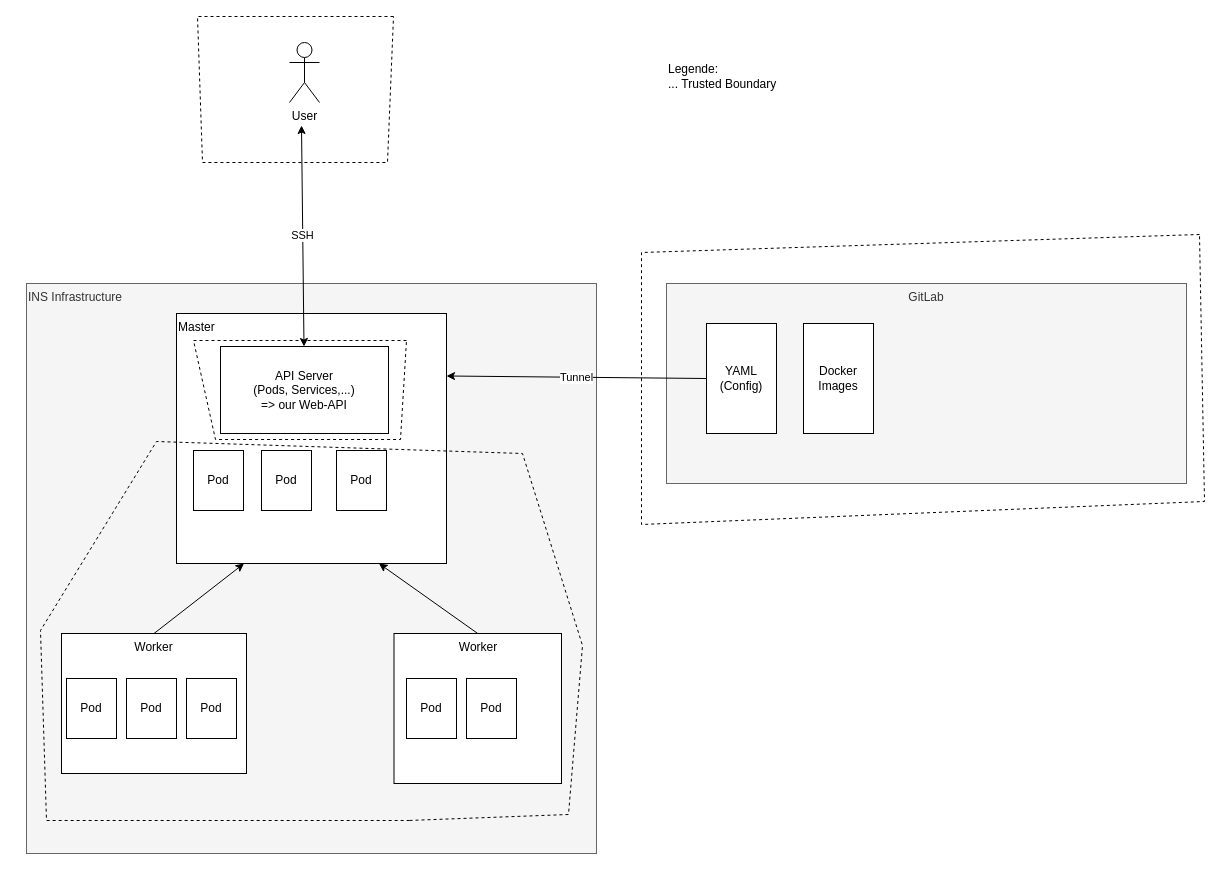
\includegraphics[height=12cm]{resources/architecture_threat_model.png}
\end{figure}
Legend: \newline
- - - Trusted Boundaries


\newpage
\section{Threat Identification}
The following table includes all threats that we found in our architecture, categorized according the STRIDE model.
\begin{longtable}[h!]{p{2.1cm} | p{1.8cm} | p{3cm} | p{2cm} | p{3.5cm}}
    \textbf{Component} & \textbf{Category} & \textbf{Threats} & \textbf{Risk} & \textbf{Mitigation} \\ \hline
    \endhead
    \caption{\label{tab:threats-classification}Classification of identified threats}
    \endlastfoot
    Frontend (incl. User)              
                        & D, E & Worm & Low & Anti-virus / Anti-malware\\
    \hline
    Frontend  \(\leftrightarrow\) KubeWatch Backend API
                        & T & Redirects Data Flow & Low & Use certificate on web server \\
                        & I & Eavesdropping & High & Encryption \\
                        & I & Verbose Exception & Medium & Correct exception handling, no critical information disclosure \\
                        & D & Botnet Attack & High & CDN and redundant system \\
    \hline
    KubeWatch Backend API
                        & S & Session Hijacking & Medium & Install SSL certificate \\
                        & T & XSS & Medium & Input validation, alert system, sanitisation \\
                        & T, I & NoSQL and PromQL Injection & High & Input validation \\
                        % & R & Audit Log Deletion & Low & Backup audit log \\ % to be added once user logs are collected
                        & I & Verbose Exception & Medium & Correct exception handling, no critical information disclosure \\
                        & D & Server Defacement & Low & ACL and Filtering \\
                        & D & Botnet Attack & High & CPU limitation, CDN and redundant system \\
                        &all& NPM Supply Chain Attack & High & Use npm audit, npm doctor, npm outdated to check for unsafe packages \\
    \hline
    KubeWatch Backend API \(\leftrightarrow\) Database
                        & T & Change Packet content & Medium & Signature, HMAC \\
                        & I & Eavesdropping & High & Encryption \\
                        & I & Verbose Exception & Medium & Correct exception handling, no critical information disclosure \\
    \hline
    Database            & T, I & NoSQL Injection & High & Input validation \\
                        % & R & Audit Log Deletion & Low & Backup audit log \\ % to be added once user logs are collected
                        % & R & Insecure Backup & Low & Implement digital signature and encryption \\
                        & I & Verbose Exception & Medium & Correct exception handling, no critical information disclosure \\
                        & D & Query Flooding & High & CPU limitation, CDN and redundant system \\
    \hline
    KubeWatch Backend API \(\leftrightarrow\) Prometheus
                        & T & Change Packet content & Medium & Signature, HMAC \\
                        & I & Eavesdropping & High & Encryption \\
    \hline
    Prometheus          & S & Session Hijacking & Low & Install SSL certificate \\
                        & T & Metrics manipulation & Low & Use secure channel / tunnel \\
                        % & R & Audit Log Deletion & Low & Backup audit log \\
                        % & R & Insecure Backup & Low & Implement digital signature and encryption \\
                        & D & Query Flooding & High & CPU limitation, CDN and redundant system \\
    \hline
\end{longtable}


\section{Model Assumptions and Explanations}

\subsection{Frontend (incl. User)}
\begin{itemize}
    \item Assumption: While KubeWatch currently does not feature a user login, a user has unrestricted access to the web application.
\end{itemize}


\subsection{Interface: Frontend \(\leftrightarrow\) KubeWatch Backend API}
\begin{itemize}
    \item Assumption: the web app can only be launched locally from a developer's IDE, provided the developer has access to the KubeWatch code on GitLab.
\end{itemize}

\subsection{KubeWatch Backend API}
\begin{itemize}
    \item The KubeWatch Backend under a DoS attack would prevent the API and the server from running
        \begin{itemize}
            \item This is a dependency on the Master
            \item Mitigation: CPU limitation and alert to users
        \end{itemize}
    \item NPM supply chain attack: a library, or a dependency, used for developing KubeWatch and for querying Prometheus could be malicious.
        \begin{itemize}
            \item Various attacks are possible under this scheme, most notably would be malware deployment.
            \item To mitigate many attack vectors, npm offers features to detect outdated or vulnerable packages, such as npm audit, npm outdated, npm doctor
        \end{itemize} 
    \item NoSQL Injection between Web App and database: mainly information disclosure, potentially Tampering to misrepresent the state of the nodes which are under a denial of service attack. This could pretend that the nodes are up and healthy, while the cluster is actually going down. However, the likelihood of this type of attack is rather low as it is questionable what the benefits are for an attacker. Unless there is a critical application running that may be the target.  
\end{itemize}

\subsection{Interface: KubeWatch Backend API \(\leftrightarrow\) Database}
No assumptions.

\subsection{Database}
\begin{itemize}
    \item We use MongoDB as a database, which uses NoSQL.
\end{itemize}


\subsection{Interface: KubeWatch Backend API \(\leftrightarrow\) Prometheus}
No assumptions.

\subsection{Prometheus}
\begin{itemize}
    \item Prometheus is an external dependency, but we need to monitor the application if any vulnerabilities appear.
    \item They implement their own query language, PromQL.
\end{itemize}